\documentclass[crop=false, class=book]{standalone}

%impostazioni lingua
\usepackage[T1]{fontenc}
\usepackage[utf8]{inputenc}
\usepackage[english,italian]{babel}

\usepackage[dvipsnames]{xcolor}
\usepackage{listings}

\lstdefinelanguage{Kotlin}{
	comment=[l]{//},
	commentstyle={\color{gray}\ttfamily},
	emph={[1]first, firstOrNull, forEach, lazy, map, mapNotNull, println},
	emphstyle={[1]\color{OrangeRed}},
	identifierstyle=\color{black},
	keywords={!in, !is, abstract, actual, annotation, as, as?, break, by, catch, class, companion, const, constructor, continue, crossinline, data, delegate, do, dynamic, else, enum, expect, external, false, field, file, final, finally, for, fun, get, if, import, in, infix, init, inline, inner, interface, internal, is, lateinit, noinline, null, object, open, operator, out, override, package, param, private, property, protected, public, receiveris, reified, return, return@, sealed, set, setparam, super, suspend, tailrec, this, throw, true, try, typealias, typeof, val, var, vararg, when, where, while, it},
	keywordstyle={\color{NavyBlue}\bfseries},
	morecomment=[s]{/*}{*/},
	morestring=[b]",
	morestring=[s]{"""*}{*"""},
	ndkeywords={@Deprecated, @JvmField, @JvmName, @JvmOverloads, @JvmStatic, @JvmSynthetic, Array, Byte, Double, Float, Int, Integer, Iterable, Long, Runnable, Short, String, Any, Unit, Nothing, Config, LightEstimationMode, CameraConfigFilter, CameraConfig, FacingDirection, AugmentedFaceMode, AugmentedFace, TrackingState, RegionType, CloudAnchorMode,AugmentedImageDatabase, BitmapFactory, Session, InstantPlacementMode, File, Uri, RecordingConfig },
	ndkeywordstyle={\color{BurntOrange}\bfseries},
	sensitive=true,
	stringstyle={\color{ForestGreen}\ttfamily},
	emph={[2]FRONT,MESH3D,ENVIRONMENTAL\_HDR,AMBIENT\_INTENSITY, DISABLED,FOREHEAD\_LEFT,FOREHEAD\_RIGHT,NOSE\_TIP, TRACKING, ENABLED, LOCAL\_Y\_UP},
	emphstyle={[2]\color{Purple}\ttfamily},
}

\definecolor{lightgrey}{RGB}{230,237,244}

\lstset{
	basicstyle=\scriptsize\sffamily\color{black},
	backgroundcolor=\color{lightgrey},
	frame=single,
	numbers=left,
	numbersep=5pt,
	numberstyle=\tiny\color{gray},
	showspaces=false,
	showstringspaces=false,
	tabsize=1,
	texcl=true,
	captionpos=b,
	breaklines=true
}




%sistema i margini
\usepackage{geometry}
\geometry{a4paper,top=2.2cm,bottom=2.2cm,left=3cm,right=3cm, heightrounded}

%interlinea 1.5
\usepackage{setspace}
\onehalfspacing

%formattazione titoli paragrafo
\usepackage{titlesec}
\titleformat{\chapter}[block]{\normalfont\huge\bfseries}{\thechapter.}{0.7em}{\huge}

%pacchetti per i riferimenti in bibliografia
\usepackage[autostyle,italian=guillemets]{csquotes}
\usepackage[sorting=none,style=numeric,citestyle=numeric-comp,backend=biber]{biblatex}
\usepackage[pdftex]{graphicx} 

%risorsa che contiene la bibliografia
\addbibresource{./../../bibliografia.bib}

\usepackage[italian]{varioref}


\begin{document}
	\chapter{Instant Placement}
	L'API di posizionamento istantaneo consente di posizionare gli oggetti nell’ambiente prima ancora che venga spostato il dispositivo e che vengano individuati i piani.
	
	Dopo che l’utente ha posizionato l’oggetto, la sua posizione viene perfezionata in tempo reale mentre l’utente si muove nell’ambiente.
	
	Successivamente, quando ARCore è in grado di identificare con precisione l’ubicazione dell’oggetto nello spazio, viene cambiata la sua posizione e dimensione per rispettare la scala dell’ambiente.
	\begin{center}
	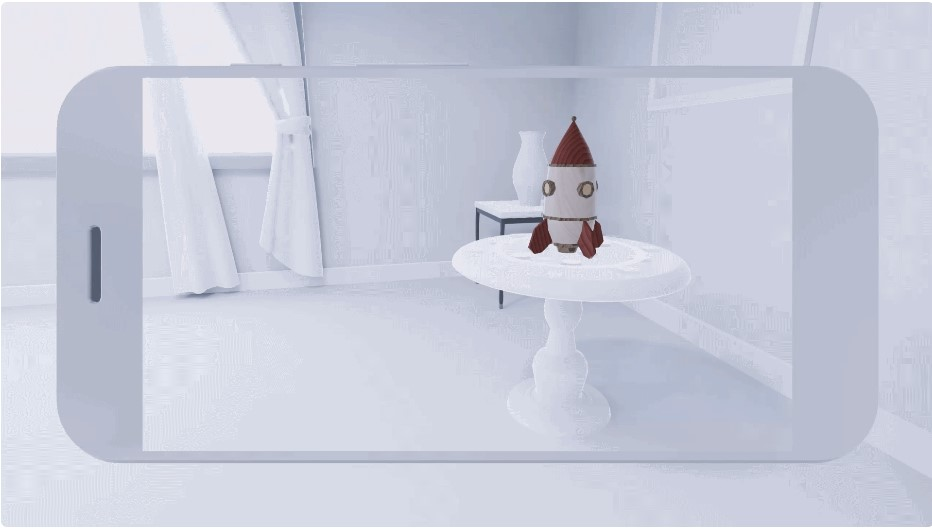
\includegraphics[scale=0.7]{InstantPlacementImg.jpg} 
	\end{center}
	\section{Abilitare Instant Placement}
	Per abilitare l’instant placement bisogna creare una sessione configurata per supportare l’instant placement, come descritto dal listing~\vref{lst:ip_session}
		
	\begin{center}
		\begin{minipage}{0.95\textwidth}
		\begin{lstlisting}[caption={Descrizione del listing.}, label={lst:ip_session}, language=Kotlin]
		fun createSession() {
		
			val session = Session(applicationContext);
			
			val config = Config(session)
			
			// Set the Instant Placement mode.
			
			config.instantPlacementMode = Config.InstantPlacementMode.LOCAL_Y_UP
			
			session.configure(config)
		}
		\end{lstlisting}
		\end{minipage}
	\end{center}

\end{document}